\documentclass{article}
\textheight = 23cm % largo texto impreso
\textwidth = 16.5cm % ancho texto impreso
\topmargin = -2cm % margen superior 3-2=1cm
\oddsidemargin = 0cm % margen izquierdo 4.5-2=2.5cm
\parindent = 4mm  % Sangría=0mm

\markright{Práctica 1}

\usepackage[spanish]{babel}
\usepackage{amsmath,amssymb,amsfonts,latexsym}
\usepackage[T1]{fontenc}
\usepackage[utf8]{inputenc}
\usepackage{multicol
\usepackage{xcolor}

\definecolor{codegreen}{rgb}{0,0.6,0}
\definecolor{codegray}{rgb}{0.5,0.5,0.5}
\definecolor{codepurple}{rgb}{0.58,0,0.82}
\definecolor{backcolour}{rgb}{0.95,0.95,0.92}

\usepackage{epsfig}
\usepackage{graphicx}
\usepackage{caption}
\usepackage{tikz}
\usetikzlibrary{shapes.geometric, arrows}
\graphicspath{ {images/} }
\usepackage{listings}
\usepackage{color}



\lstdefinestyle{mystyle}{
    backgroundcolor=\color{backcolour},   
    commentstyle=\color{codegreen},
    keywordstyle=\color{magenta},
    numberstyle=\tiny\color{codegray},
    stringstyle=\color{codepurple},
    basicstyle=\ttfamily\footnotesize,
    breakatwhitespace=false,         
    breaklines=true,                 
    captionpos=b,                    
    keepspaces=true,                 
    numbers=left,                    
    numbersep=5pt,                  
    showspaces=false,                
    showstringspaces=false,
    showtabs=false,                  
    tabsize=2
}

\lstset{style=mystyle}
\renewcommand{\thesection}{\Roman{section}}
\renewcommand{\thesubsection}{\arabic{subsection}}
%------------------------
\begin{document}

\title{\Large Instituto Politécnico Nacional\\
   {\large {\fontfamily{bch}\selectfont 
   			{\large Unidad Profesional Interdisciplinaria en Ingeniería y Tecnologías Avanzadasl}\\
   				{\large  Ingeniería biónica }\\
   				{\normalsize Programación orientada a objetos}\\
   			 
   			{\large Práctica 1: Minipunto de venta}\\
   		}
   }}
   \author{Archundia Bazán Aarón Antonio,\\ Guerrero Vélez Eliseo Milton,\\ Hernández Vázquez Cesar Arturo}
\date{26 de octubre de 2020}
\maketitle


	\begin{center}
 \section{ Planteamiento del problema}
     \end{center}


        Se precisa elaborar un sistema de punto de venta que le permita al usuario o al empleado que lo desee, generar tickets a partir de los productos disponibles y sus respectivos costos. Hay cinco productos seleccionables en la tienda con cinco precios diferentes enumerados en el cuadro 1:\\\\
\begin{center}
        \begin{tabular}{|c|c|c}
                \hline
                Producto  & Precio \\
                \hline
                Producto 1 & \$2.98 \\
                \hline
                Producto 2 & \$4.50 \\
                \hline
                Producto 3  & \$9.98 \\
                \hline
                Producto 4 & \$4.49  \\
                \hline
                Producto 5  & \$6.87 \\
                \hline
        
        \end{tabular}
\captionof{table}{Productos disponibles con sus precios}\label{table4}     
\end{center}


\begin{center}
\section{Propuesta de Solución}
    	\end{center}
    Para solucionar el problema se propuso calcular la sumatoria total de artículos comprados; realizando el producto del precio de cada artículo por su cantidad vendida.\\\\
    
                 \begin{center}
                        $VentaT = \sum (Precioproducto*Cantidadvendida)$
                 \end{center}  
        
                 Como únicamente son cinco productos, la sumatoria se haría del producto 1 hasta el producto 5.
        
                \begin{center}
                       $VentaT = \sum\limits_{N_p=1}^{N_p=5} (Precioproducto*cantidadvendida)$
                \end{center}
    
    Esto se ejecutará cíclicamente dependiendo de cuántos productos requiera comprar el usuario. Si este únicamente quiere un producto, la sentencia de control do-while permitirá que el usuario ejecute una vez y termine, pero si quiere tomar algún otro producto, continuará hasta que este termine de escoger y ordene ya no querer continuar comprando. Finalmente, se le imprimirá un ticket de compra con el total de sus gastos parciales y totales.


\begin{center}
\section{Análisis y diseño}
\subsection{Diagrama de flujo}

\subsection{Diagrama de flujo}
\begin{center}
 	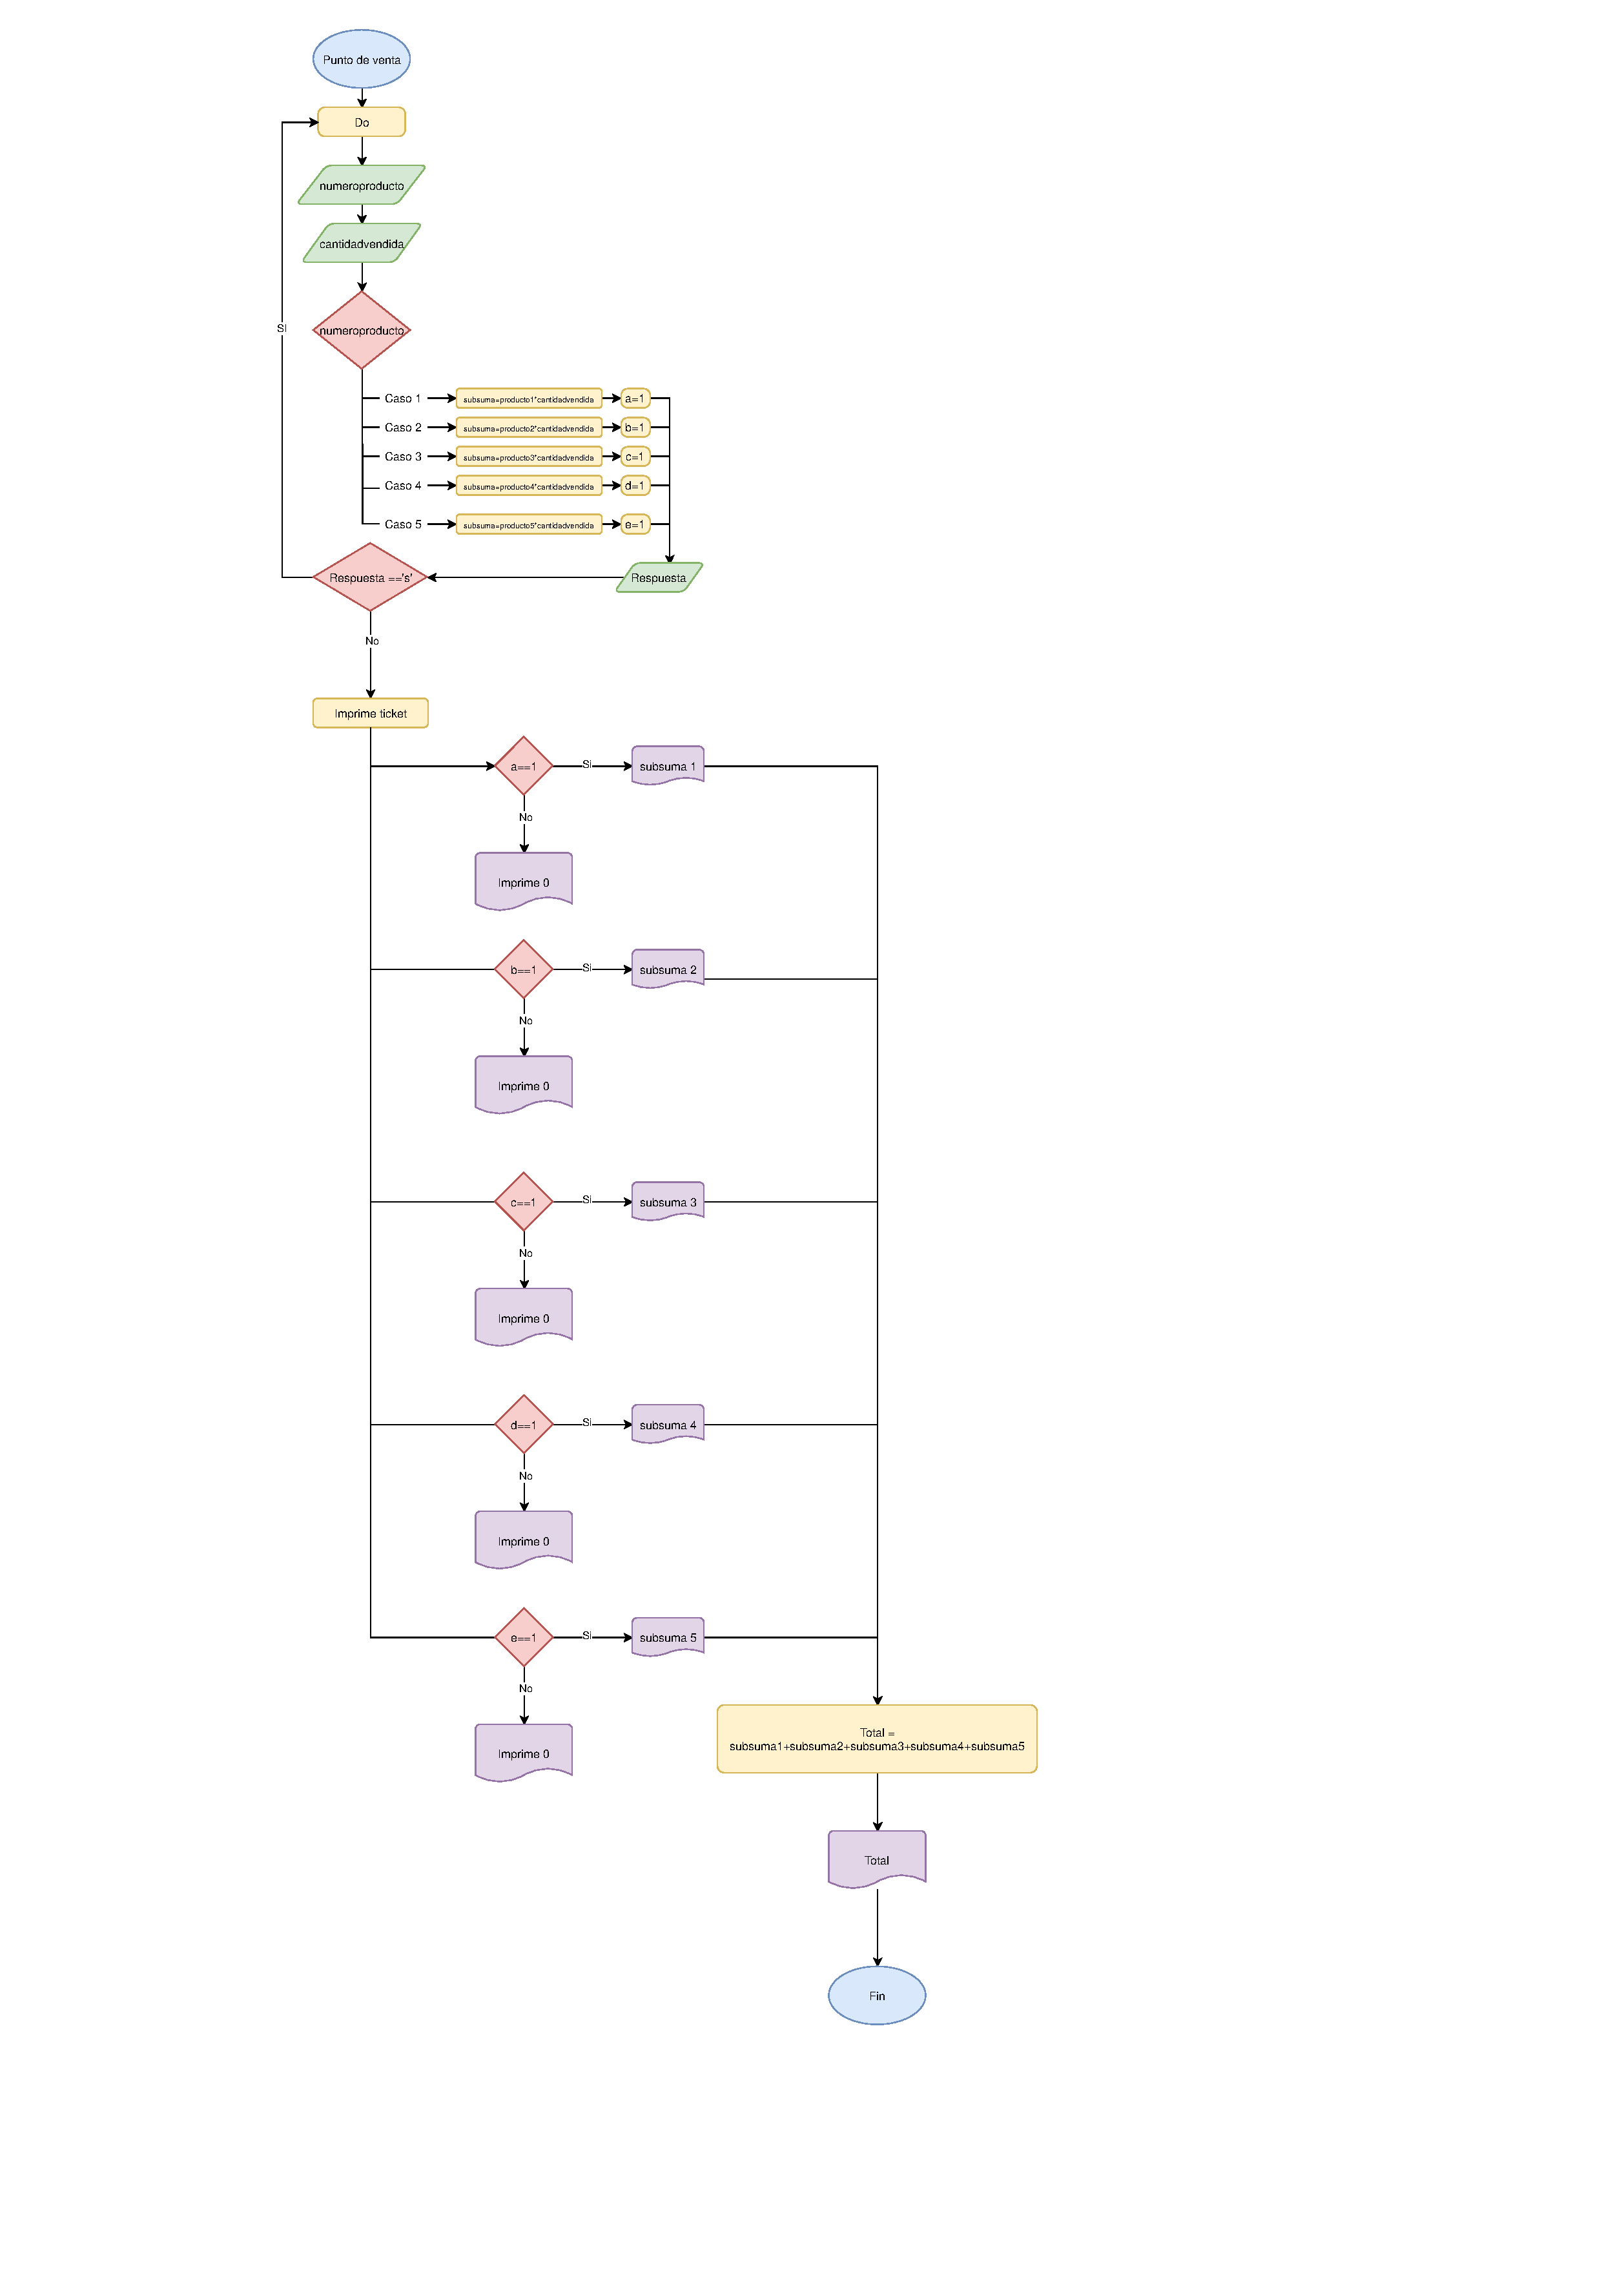
\includegraphics[scale=0.35]{images/Diagrama.eps}
 	\captionof{figure}{Diagrama de flujo, Minipunto de venta}
 	\label{figura4}
 \end{center}
\end{center}

\clearpage
\newpage

\begin{center}

\section{Implementación y pruebas}
\end{center}
    Se utilizó la plataforma GitHub para el control de versiones de nuestro minipunto de venta, donde se realizaron los cambios pertinentes con la finalidad de trabajar en equipo a distancia.\\
    
    
    \begin{center} 
	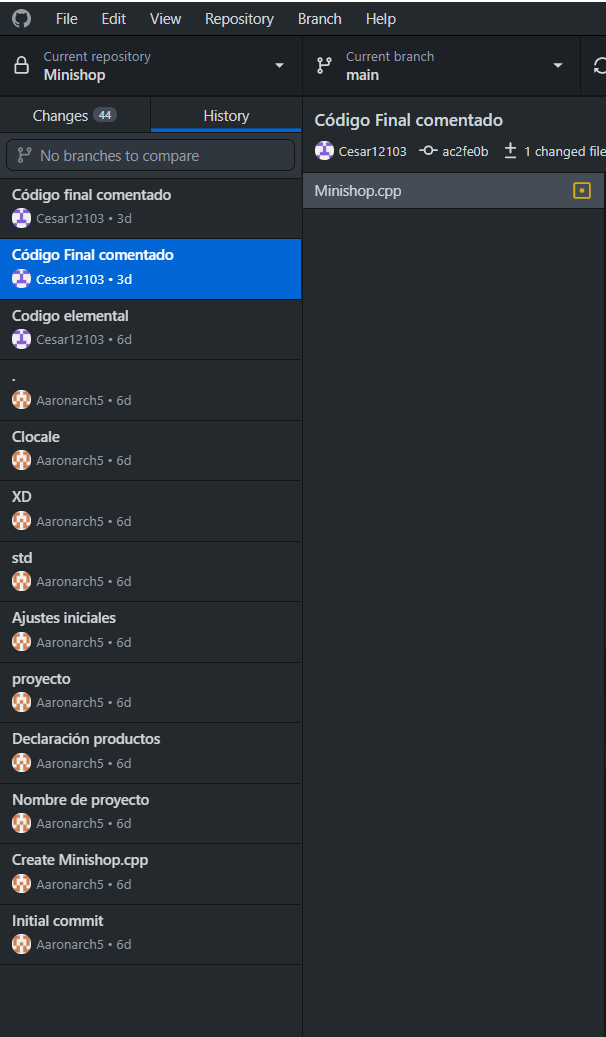
\includegraphics[scale=0.3]{Images/Captura de pantalla (213).png}
	\captionof{figure}{Cambios hechos por integrantes}
	\label{figura3a}
\end{center}


\begin{center} 
	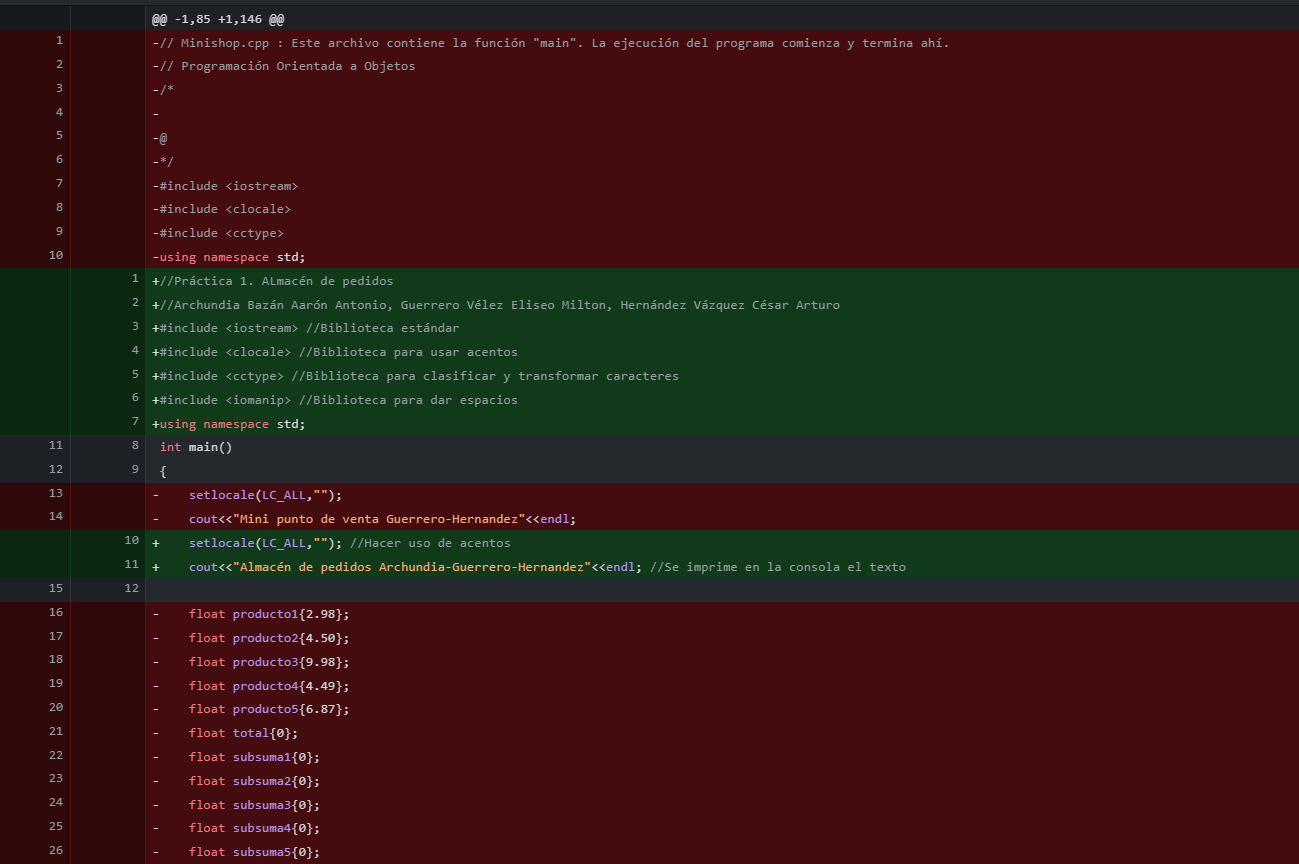
\includegraphics[scale=0.2]{Images/Captura de pantalla (214).png}
	\captionof{figure}{Cambios con el tiempo (Rojo, código borrado,Verde, código actual)}
	\label{figura3b}
\end{center}

\clearpage

\subsection*{Caso I.}
Cuando solo se requiera comprar un producto, solo se hará la multiplicación entre la cantidad de piezas y el precio unitario.      
\begin{center}
\begin{large}
        $ VentaT =  precioproducto * cantidadvendida $
\end{large}
\end{center}
        
    \begin{center} 
	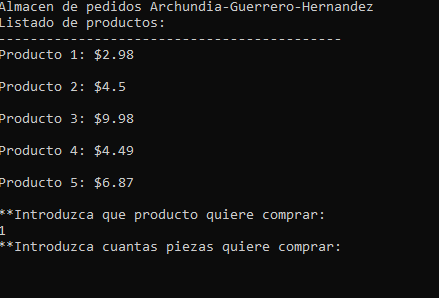
\includegraphics[scale=0.5]{Images/Paso1.PNG}
	\captionof{figure}{Paso 1: Elegir producto}
	\label{figura3C}
\end{center}

\begin{center} 
	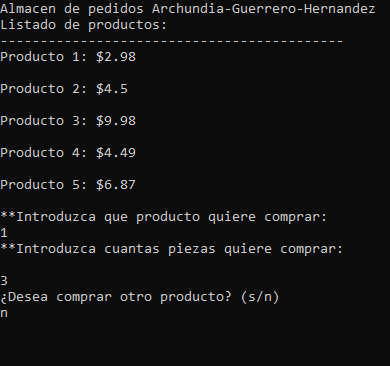
\includegraphics[scale=0.5]{Images/Paso2.PNG}
	\captionof{figure}{Paso 2: Elegir la cantidad de piezas
}
	\label{figura3D}
\end{center}

\begin{center} 
	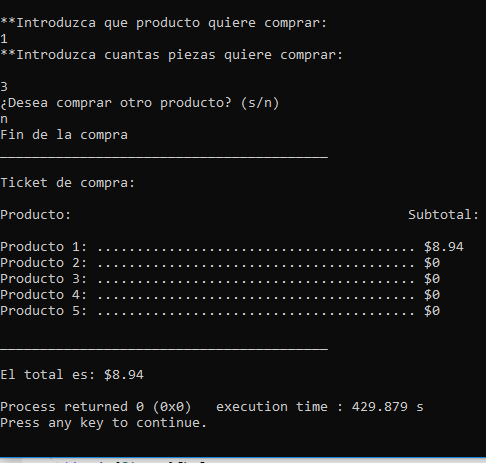
\includegraphics[scale=0.5]{Images/Paso3.PNG}
	\captionof{figure}{Paso 3: Se despliega el Ticket de compra con el precio de los productos adquiridos}
	\label{figura3E}
\end{center}

\newpage

\subsection*{Caso II.}
Cuando se va a comprar más de un artículo, el programa sumará las multiplicaciones entre la cantidad de piezas compradas con sus respectivos precios unitarios.

\begin{center}
	\begin{large}
		$VentaT = \sum\limits_{N_p=1}^{N_p=3} (Precioproducto*cantidadvendida)$
	\end{large}
\end{center}


\begin{center} 
	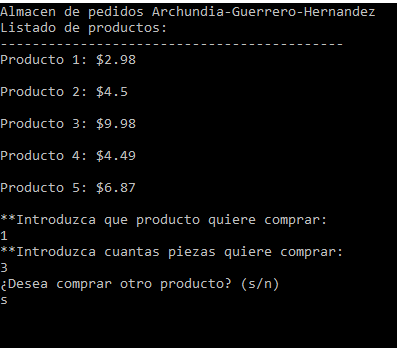
\includegraphics[scale=0.5]{Images/Paso1(2).PNG}
	\captionof{figure}{Paso 1: Elegir el primer producto y la cantidad, seguir eligiendo productos (s)}
	\label{figura3f}
\end{center}

\begin{center} 
	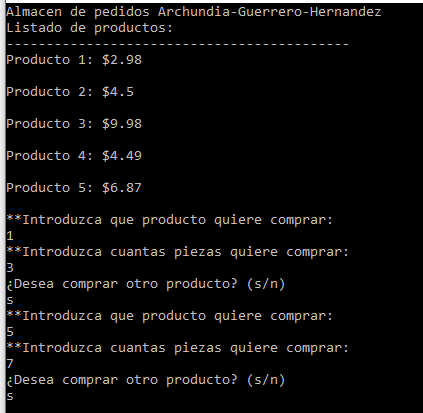
\includegraphics[scale=0.5]{Images/Paso2(2).PNG}
	\captionof{figure}{Paso 2: Elegir los siguientes productos y la cantidad de piezas, no seguir comprando productos para terminar (n) }
	\label{figura3g}
\end{center}


\begin{center} 
	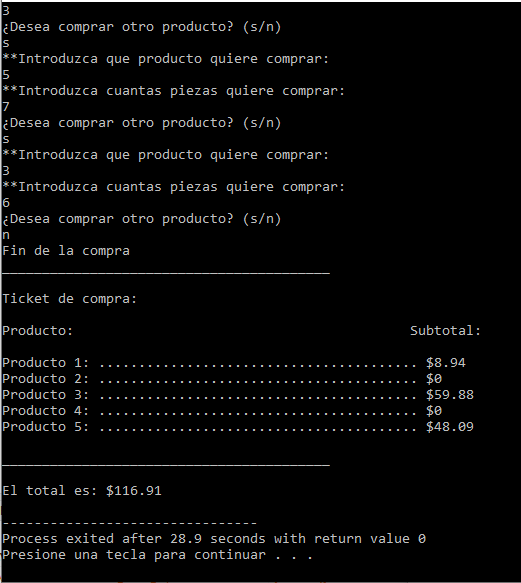
\includegraphics[scale=0.4]{Images/Paso4(2).PNG}
	\captionof{figure}{Paso 3: Se despliega el Ticket de compra con el precio total de los productos adquiridos}
	\label{figura3h}
\end{center}


\begin{center}
\section{Código fuente comentado}
\end{center}

\lstinputlisting[language=C++]{Minishop.cpp}

\newpage

\begin{center}
\section{Conclusiones}
\end{center}

Gracias a los resultados obtenidos podemos concluir que mediante el uso de bucles controlados tales como do while, de instrucciones de control como switch, además de la implementación de múltiples funciones más; podemos elaborar una herramienta útil y funcional para una problemática real, como lo es la disposición y facilitación en la elaboración de cuentas basadas en sumas y multiplicaciones, que a pesar de mostrar en este caso, valores pequeños y un "stock" limitado, este programa puede proyectarse a una cantidad mayor y generar cuentas cada vez más complejas y favorecer a la productividad y optimización de este proceso.

\end{document}
